\documentclass[12pt,oneside]{article}
\usepackage[]{mathpazo}
\usepackage{amssymb,amsmath}
\usepackage{ifxetex,ifluatex}
\usepackage{fixltx2e} % provides \textsubscript
\ifnum 0\ifxetex 1\fi\ifluatex 1\fi=0 % if pdftex
  \usepackage[T1]{fontenc}
  \usepackage[utf8]{inputenc}
\else % if luatex or xelatex
  \ifxetex
    \usepackage{mathspec}
  \else
    \usepackage{fontspec}
  \fi
  \defaultfontfeatures{Ligatures=TeX,Scale=MatchLowercase}
\fi
% use upquote if available, for straight quotes in verbatim environments
\IfFileExists{upquote.sty}{\usepackage{upquote}}{}
% use microtype if available
\IfFileExists{microtype.sty}{%
\usepackage{microtype}
\UseMicrotypeSet[protrusion]{basicmath} % disable protrusion for tt fonts
}{}
\usepackage[margin=1in]{geometry}
\usepackage{hyperref}
\PassOptionsToPackage{usenames,dvipsnames}{color} % color is loaded by hyperref
\hypersetup{unicode=true,
            pdftitle={Supplementary Material},
            pdfauthor={Issoufou Liman1,2,; Cory Whitney1,3; James Kungu2; Eike Luedeling1,3,4},
            colorlinks=true,
            linkcolor=blue,
            citecolor=red,
            urlcolor=blue,
            breaklinks=true}
\urlstyle{same}  % don't use monospace font for urls
\usepackage{longtable,booktabs}
\usepackage{graphicx,grffile}
\makeatletter
\def\maxwidth{\ifdim\Gin@nat@width>\linewidth\linewidth\else\Gin@nat@width\fi}
\def\maxheight{\ifdim\Gin@nat@height>\textheight\textheight\else\Gin@nat@height\fi}
\makeatother
% Scale images if necessary, so that they will not overflow the page
% margins by default, and it is still possible to overwrite the defaults
% using explicit options in \includegraphics[width, height, ...]{}
\setkeys{Gin}{width=\maxwidth,height=\maxheight,keepaspectratio}
\IfFileExists{parskip.sty}{%
\usepackage{parskip}
}{% else
\setlength{\parindent}{0pt}
\setlength{\parskip}{6pt plus 2pt minus 1pt}
}
\setlength{\emergencystretch}{3em}  % prevent overfull lines
\providecommand{\tightlist}{%
  \setlength{\itemsep}{0pt}\setlength{\parskip}{0pt}}
\setcounter{secnumdepth}{5}

%%% Use protect on footnotes to avoid problems with footnotes in titles
\let\rmarkdownfootnote\footnote%
\def\footnote{\protect\rmarkdownfootnote}

%%% Change title format to be more compact
\usepackage{titling}

% Create subtitle command for use in maketitle
\providecommand{\subtitle}[1]{
  \posttitle{
    \begin{center}\large#1\end{center}
    }
}

\setlength{\droptitle}{-2em}

  \title{Supplementary Material}
    \pretitle{\vspace{\droptitle}\centering\huge}
  \posttitle{\par}
  \subtitle{Modelling Risk and Uncertainty in Flood-based farming systems.}
  \author{Issoufou Liman\textsuperscript{1,2,*} \\ Cory Whitney\textsuperscript{1,3} \\ James Kungu\textsuperscript{2} \\ Eike Luedeling\textsuperscript{1,3,4}}
    \preauthor{\centering\large\emph}
  \postauthor{\par}
      \predate{\centering\large\emph}
  \postdate{\par}
    \date{May 23, 2019}

% \documentclass{article} https://tex.stackexchange.com/questions/60209/how-to-add-an-extra-level-of-sections-with-headings-below-subsubsection
\usepackage{hyperref}
\makeatletter
% Editing the default numbering style
\renewcommand{\thesection}{\Roman{section}.}
\renewcommand{\thesubsection}{\thesection\arabic{subsection}.}
\renewcommand{\thesubsubsection}{\thesubsection\arabic{subsubsection}.}

\renewcommand\paragraph{\@startsection{paragraph}{4}{\z@}%
            {-2.5ex\@plus -1ex \@minus -.25ex}%
            {1.25ex \@plus .25ex}%
            {\normalfont\normalsize\bfseries}}   

% \renewcommand\subparagraph{\@startsection{subparagraph}{5}{\z@}%
%             {-1.25ex\@plus -1ex \@minus -.30ex}%
%             {1.00ex \@plus .30ex}%
%             {\normalfont\normalsize\bfseries}}
            
\renewcommand\subparagraph{\@startsection{subparagraph}{5}{\z@}%
            {-1.25ex\@plus -1ex \@minus -.30ex}%
            {1.00ex \@plus .30ex}%
            {\normalfont\normalsize\bfseries\itshape}}  
            
\renewcommand{\theparagraph}{\thesubsubsection\arabic{paragraph}.}
\renewcommand{\thesubparagraph}{\theparagraph\arabic{subparagraph}.}


\makeatother
\setcounter{secnumdepth}{3} % how many sectioning levels to assign numbers to
\setcounter{tocdepth}{5}    % how many sectioning levels to show in ToC

\begin{document}
\maketitle
\begin{abstract}
Modelling the performance of crops grown under specific conditions is an important tool for decision support. Towards this end, many crop models are being used to inform agricultural policies. However, many of these models are applied beyond a reasonable scope of application, mainly because they are either designed for other settings, they fail to capture system complexity, or because some of their data requirements are not within reach. In this paper, we demonstrate an approach to overcome the above-mentioned problems using a probabilistic crop model based on the Decision Theory methods. Using the innovative method, we transparently use all available sources of information and consider various sources of uncertainty using participatory analysis. The transdisciplinary process provides a model where all important variables and their interactions, as determined by local experts and relevant literature, are used to simulate the plausible ranges of expected grain and biomass yield at various stages of crop development. System components are described using individual Bayesian networks in which expert knowledge is employed to specify causality among important variables along with their probability distributions. These Bayesian networks, along with other quantitative variables, are used as input for a Monte Carlo model to simulate the plausible performance of crops. Our objective is to develop a customizable solution-oriented approach for crop modelling in settings where data and resources are limited. We describe how such a model can be developed and provide three case study applications focusing on flood-based farming systems. The case studies illustrate the extensible scope of such a model by assessing the performance of a cropping system, individual crops, or other factors of high agricultural importance across the Tigray region of Ethiopia and Kisumu County of Kenya. The probabilistic tools and transdisciplinary approaches of Decision Theory allow experts and analysts to address the system complexity and data uncertainties in crop modelling.
\end{abstract}

{
\hypersetup{linkcolor=black}
\setcounter{tocdepth}{5}
\tableofcontents
}
\textsuperscript{1} World Agroforestry Centre (ICRAF), United Nations Avenue, Gigiri, P. O. Box 30677-00100, Nairobi, Kenya\\
\textsuperscript{2} Kenyatta University, Department of Environmental Sciences\\
\textsuperscript{3} Center for Development research (ZEF), University of Bonn, Genscherallee 3, D-53113, Bonn, Germany\\
\textsuperscript{4} University of Bonn, Department of Horticultural Sciences, Auf dem Hügel 6, D-53121, Bonn, Germany

\textsuperscript{*} Correspondence: \href{mailto:issoufoul@gmail.com}{Issoufou Liman \textless{}\href{mailto:issoufoul@gmail.com}{\nolinkurl{issoufoul@gmail.com}}\textgreater{}}

\hypertarget{I}{%
\section{Introduction}\label{I}}

A complex crop model was developed for Flood-based Farming Systems across the Kisumu County in Kenya and Tigray region in Ethiopia. This document provides supplementary materials supporting some of the claims made in the result section of the main paper.

\hypertarget{II}{%
\section{Result}\label{II}}

\hypertarget{bayesian-networks-models-ii1}{%
\subsection{Bayesian Networks Models \{\# II1\}}\label{bayesian-networks-models-ii1}}

\hypertarget{I11}{%
\subsubsection{Farming Constraints at farming plot level}\label{I11}}

A BN describing the farming constraints in presented in Figure 1. The most important limiting factors describing the farming constraints in the study areas the adequacy of water supply to crops (AdeqWatSupl), the effectiveness of cropping systems (EffCropSystems), and the quality of farming practices (AgricManagEff) resulting from farmers' managements options (Figure 2 to Figure 6). These will be described in more details in sections I.1.2 to I.1.4.

\begin{figure}[!htbp]

{\centering 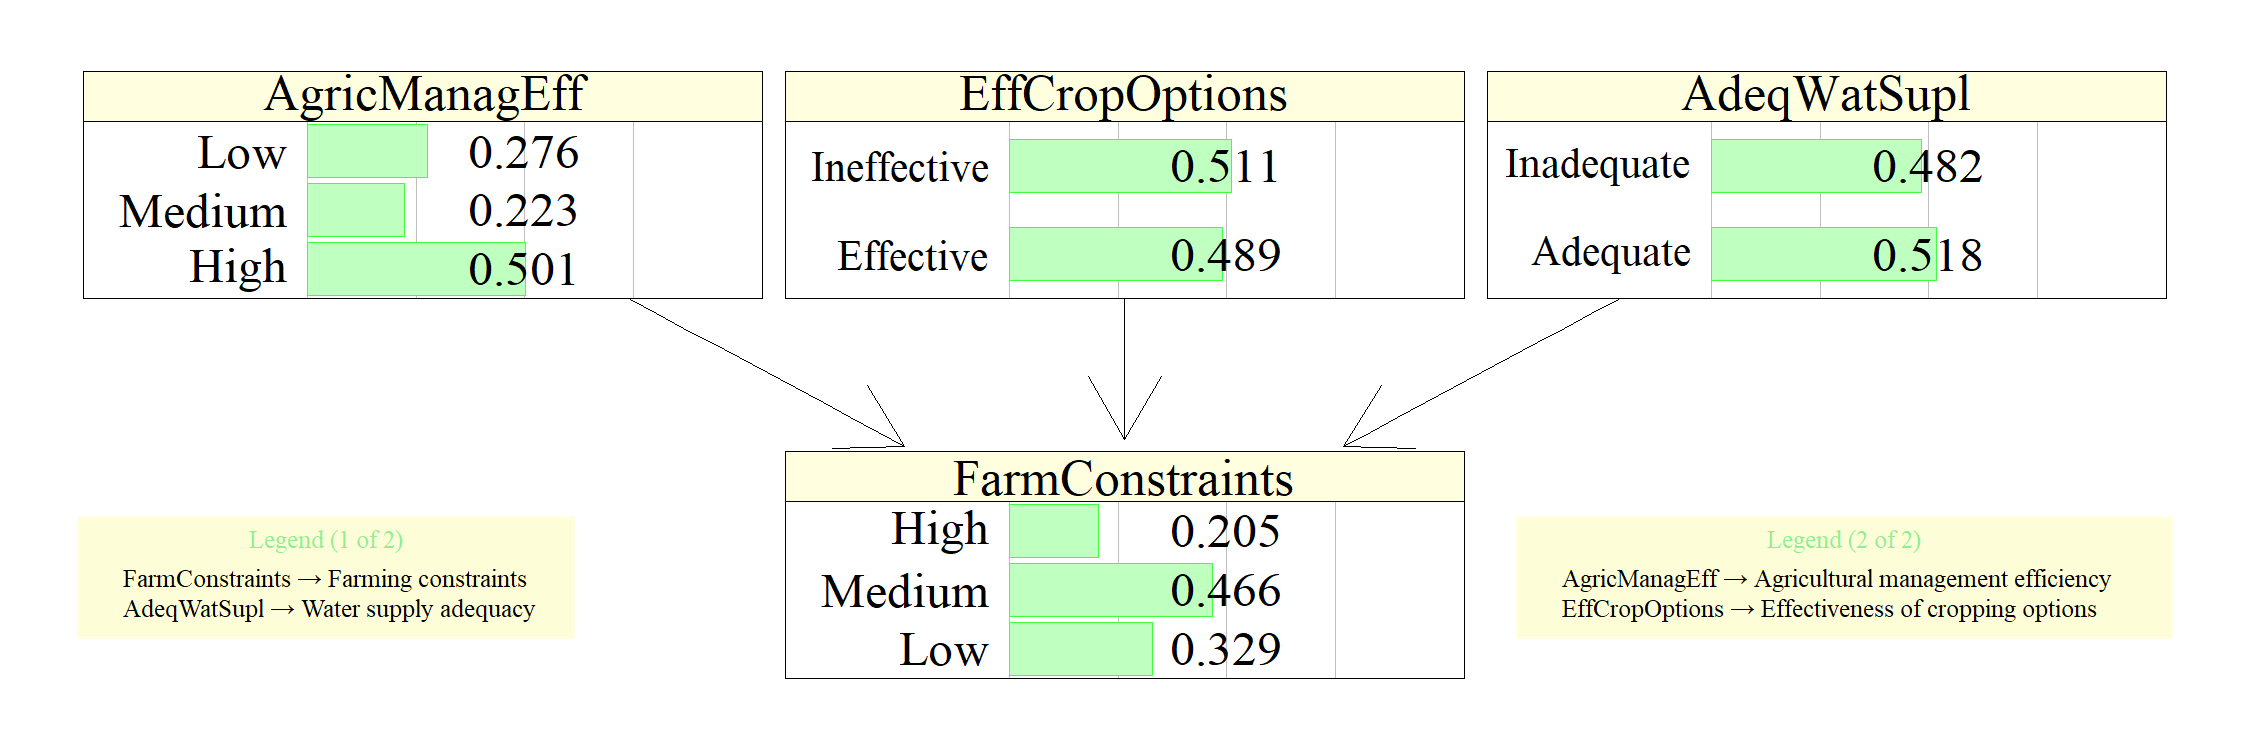
\includegraphics[width=1\linewidth,]{figures/Modelling_FBFS_Suppl_Farming_Constraints_BNs_plot} 

}

\caption{BNs describing important variables as part of a mixed model describing the farming constraints in FBFS in Kisumu (Kenya) and Tigray (Ethiopia).}\label{fig:fig1}
\end{figure}

\hypertarget{water-supply-adequacy-i12}{%
\subsubsection{Water Supply Adequacy \{\# I12\}}\label{water-supply-adequacy-i12}}

A BN describing the processes leading to the amount of flood reaching the plot (FloodReachsPlot) is presented in Figure 2. The amount of flood reaching the farming plot was assessed separately since it is an important variable with regards to the overall available water for crop development under FBFS setting.

\begin{figure}[!htbp]

{\centering 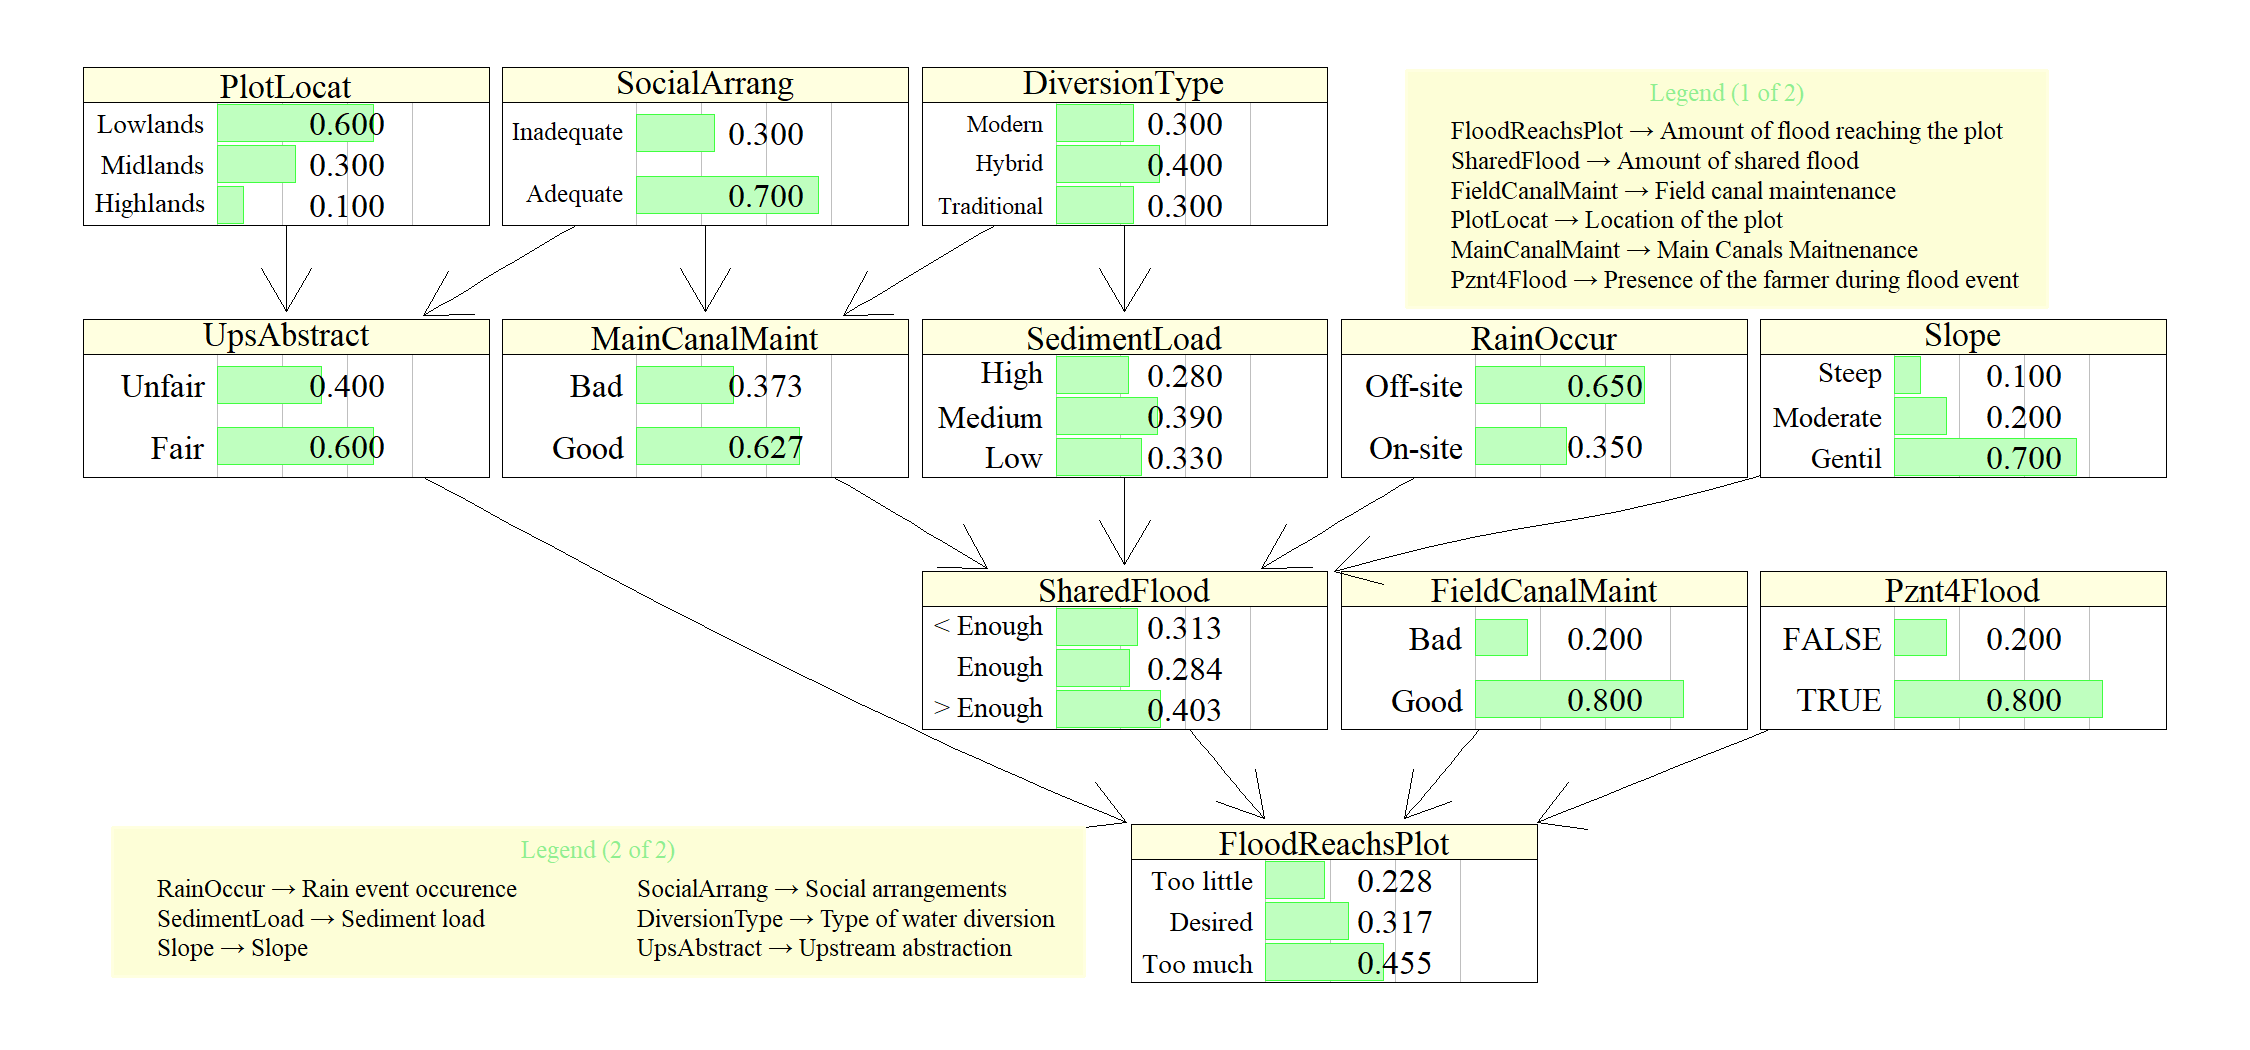
\includegraphics[width=1\linewidth,]{figures/Modelling_FBFS_Suppl_flood_reaching_plot_BNs_plot} 

}

\caption{BNs describing important variables as part of a mixed model describing the amount of flood at the farming plot level in FBFS in Kisumu (Kenya) and Tigray (Ethiopia).}\label{fig:fig2}
\end{figure}

At the root of the amount of flood reaching the plot BNs are the nodes describing water diversion type (DiversionType), the social arrangement for water acquisition and sharing (SocialArrang), and the location of the farming plot (PlotLocat). The water diversion type is important since it determines the overall water delivery (SharedFlood) and ultimately the overall expected flood amount at the plot level (FloodReachsPlot) via the way in which farmers are committed as a group (SocialArrang) to maintain their main water distribution networks (MainCanalMaint) and its efficiency with regards to sediment budget (SedimentLoad). If the social organisation (SocialArrang) is not adequate along a topographic gradient (Slope), it may lead to unfair upstream abstraction (UpsAbstract), hence penalising water users downstream (FloodReachsPlot). Flood water is trapped in FBFS using earthen bunds (Figure 1; Main) which need to be close/open at the right time either for irrigation if need or water release if too much. Individual farmers, therefore, need to make sure this happens by being present at the right time and making sure the water is diverted from the main canal to their respective secondary and tertiary sub-water distribution system. Given the adequacy of the above-mentioned aspects, farmers presence in the field during floods (Pznt4Flood) and the quality of their maintenance of the canals (FieldCanalMaint) can still strongly affect the amount of flood reaching their plot (FloodReachsPlot), and ultimately the overall soil water budget. These may have minor importance when there is rainfall on the field (RainOccur = On-site) and major importance in the case of spontaneous flood event from upstream (RainOccur = Off-site).

\begin{figure}[!htbp]

{\centering 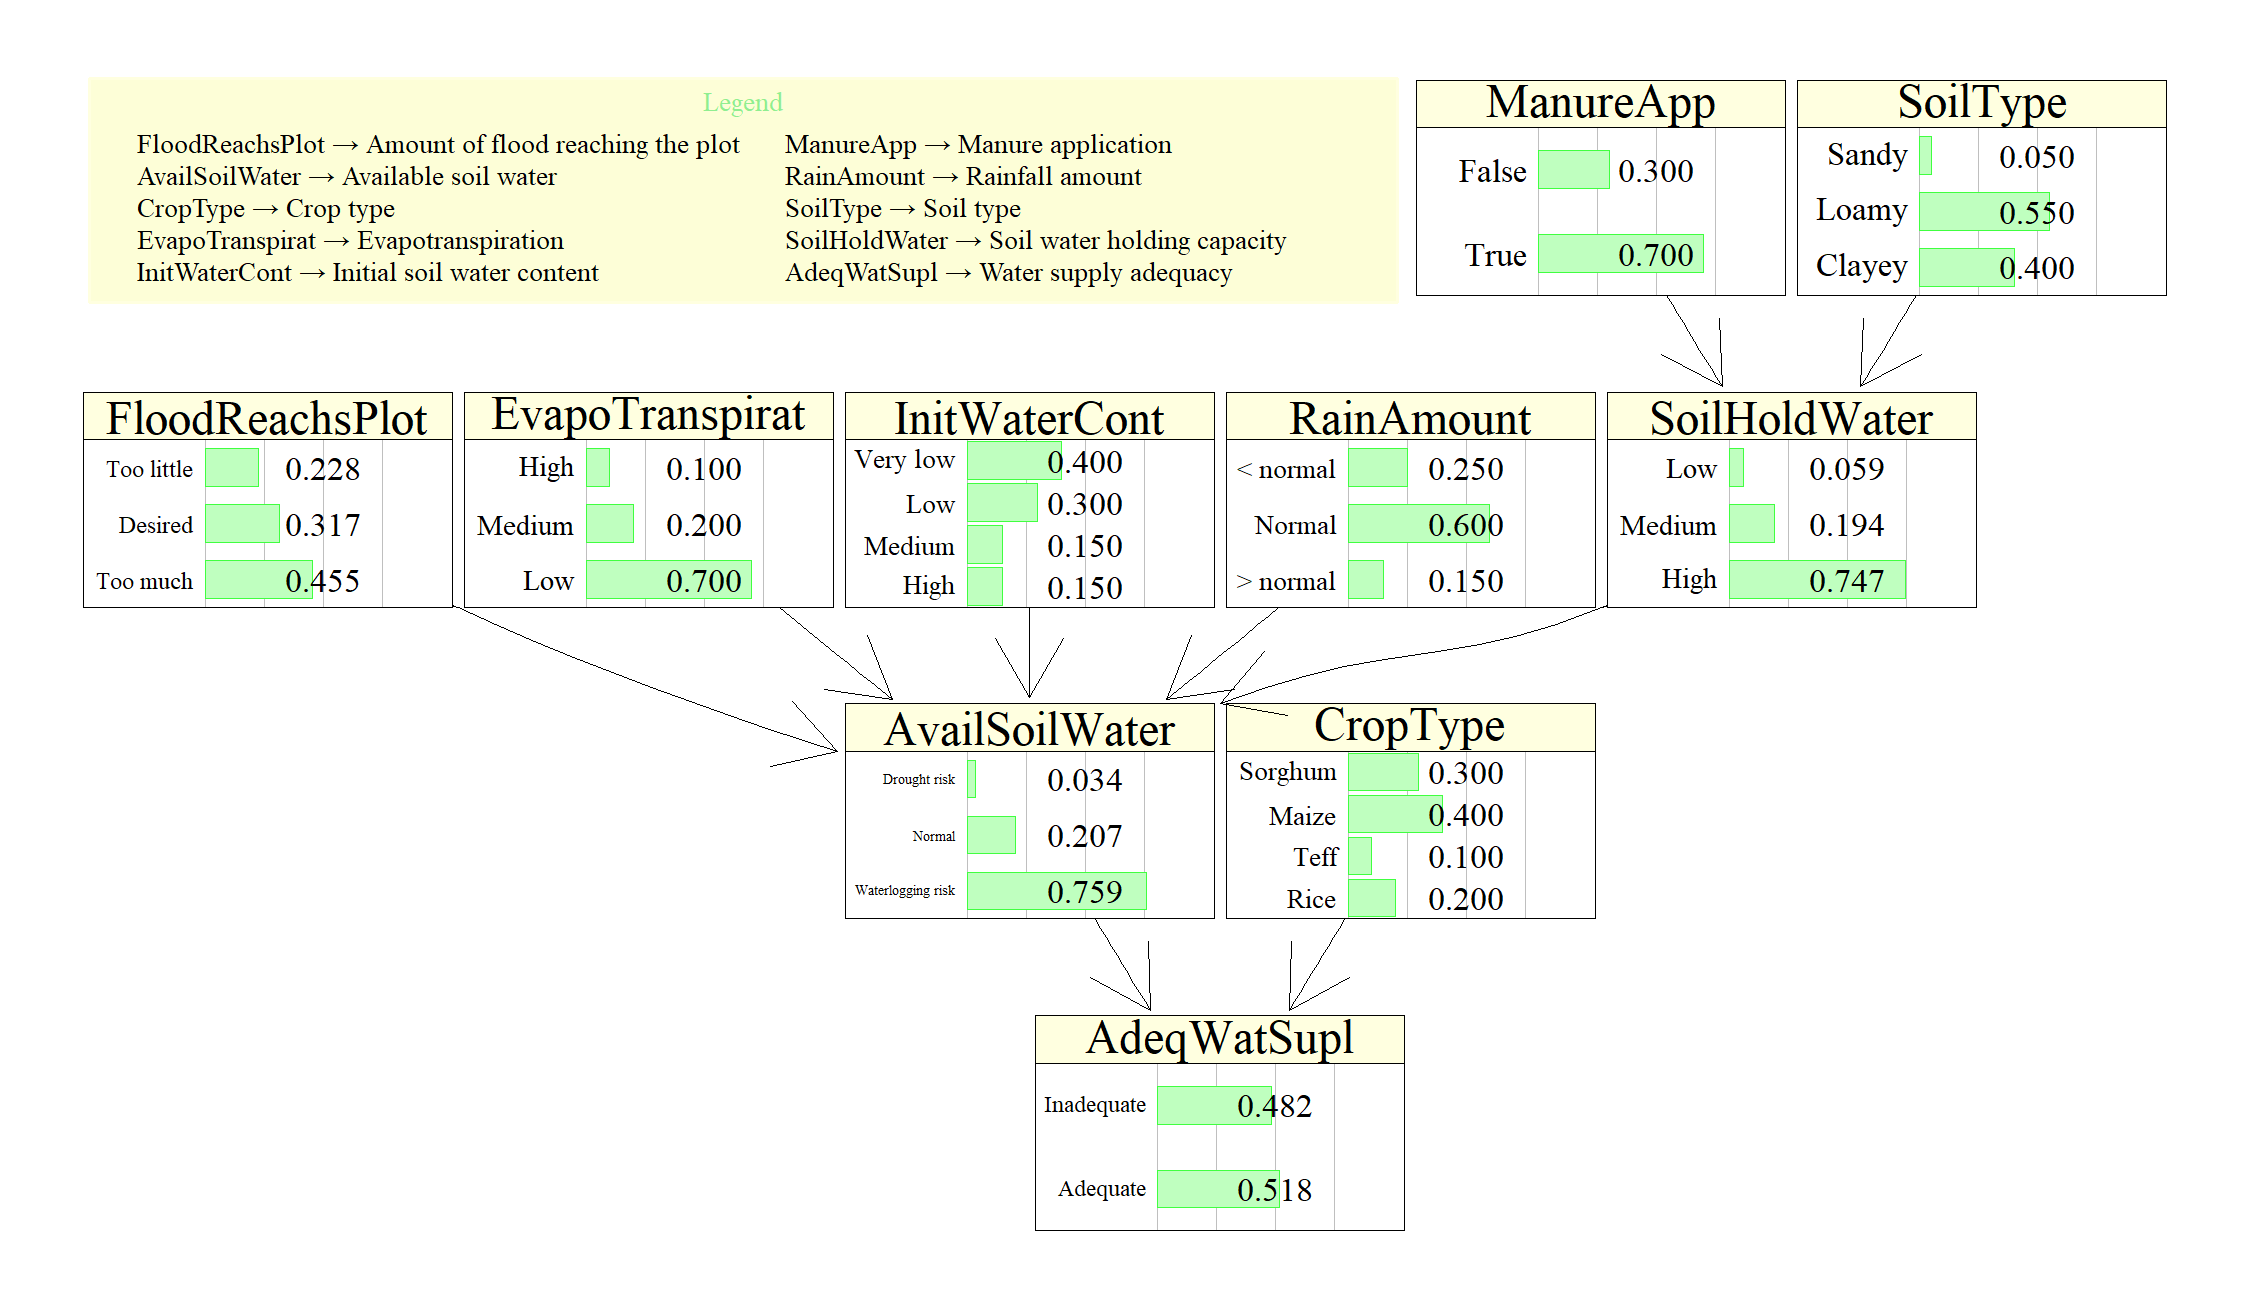
\includegraphics[width=1\linewidth,]{figures/Modelling_FBFS_Suppl_Water_Supply_Adequacy_BNs_plot} 

}

\caption{BNs describing important variables as part of a mixed model describing the water supply adequacy in FBFS in Kisumu (Kenya) and Tigray (Ethiopia).}\label{fig:fig3}
\end{figure}

The soil water profile of a given farming plot includes important biophysical aspects related to soils and climate. The available water for crops is determined by the soil water holding capacity (SoilHoldWater), the total amount and temporal distribution of rainfall (RainAmount) along with residual soil moisture (InitWaterCont), which can be significant under certain FBFS such as flood recession agriculture. Soil water holding capacity (SoilHoldWater) can vary greatly depending on the soil type (SoilType), and the soil management strategies employed by the farmer (e.g.~manure application (ManureApp).

\hypertarget{I13}{%
\subsubsection{Agricultural management efficiency}\label{I13}}

A BN describing the process that can lead to farming inefficiency (FarmingIneff) is presented using two graphs, one (Figure 4) describing the available soil nutrient (AvailSoilNut), and the other (Figure 5) describing the overall agricultural management efficiency. The amount of available soil nutrients is defined by the fertilizer applications either in the form of organic (ManureApp) or mineral addition (FertiApp) by the farmer, and on the other hand by the sediment naturally brought by the flood water. Here, it is important to distinguish between coarse sediments (SedimentLoad) described under the rubric Available soil water which are likely to have negative impact and the fine rich sediments (AddSediments) which have positive impact on crops. Fertilizer application can only be expected when the desired fertilizer by the farmer is available on the market at the time when the farmers can afford it (Access2Inputs). This depends on the purchasing power of farmers and their willingness to acquire the fertilizers (RelativeWealth) in the one hand and the mutual aids (MutualAids) among peer farmers.

\begin{figure}[!htbp]

{\centering 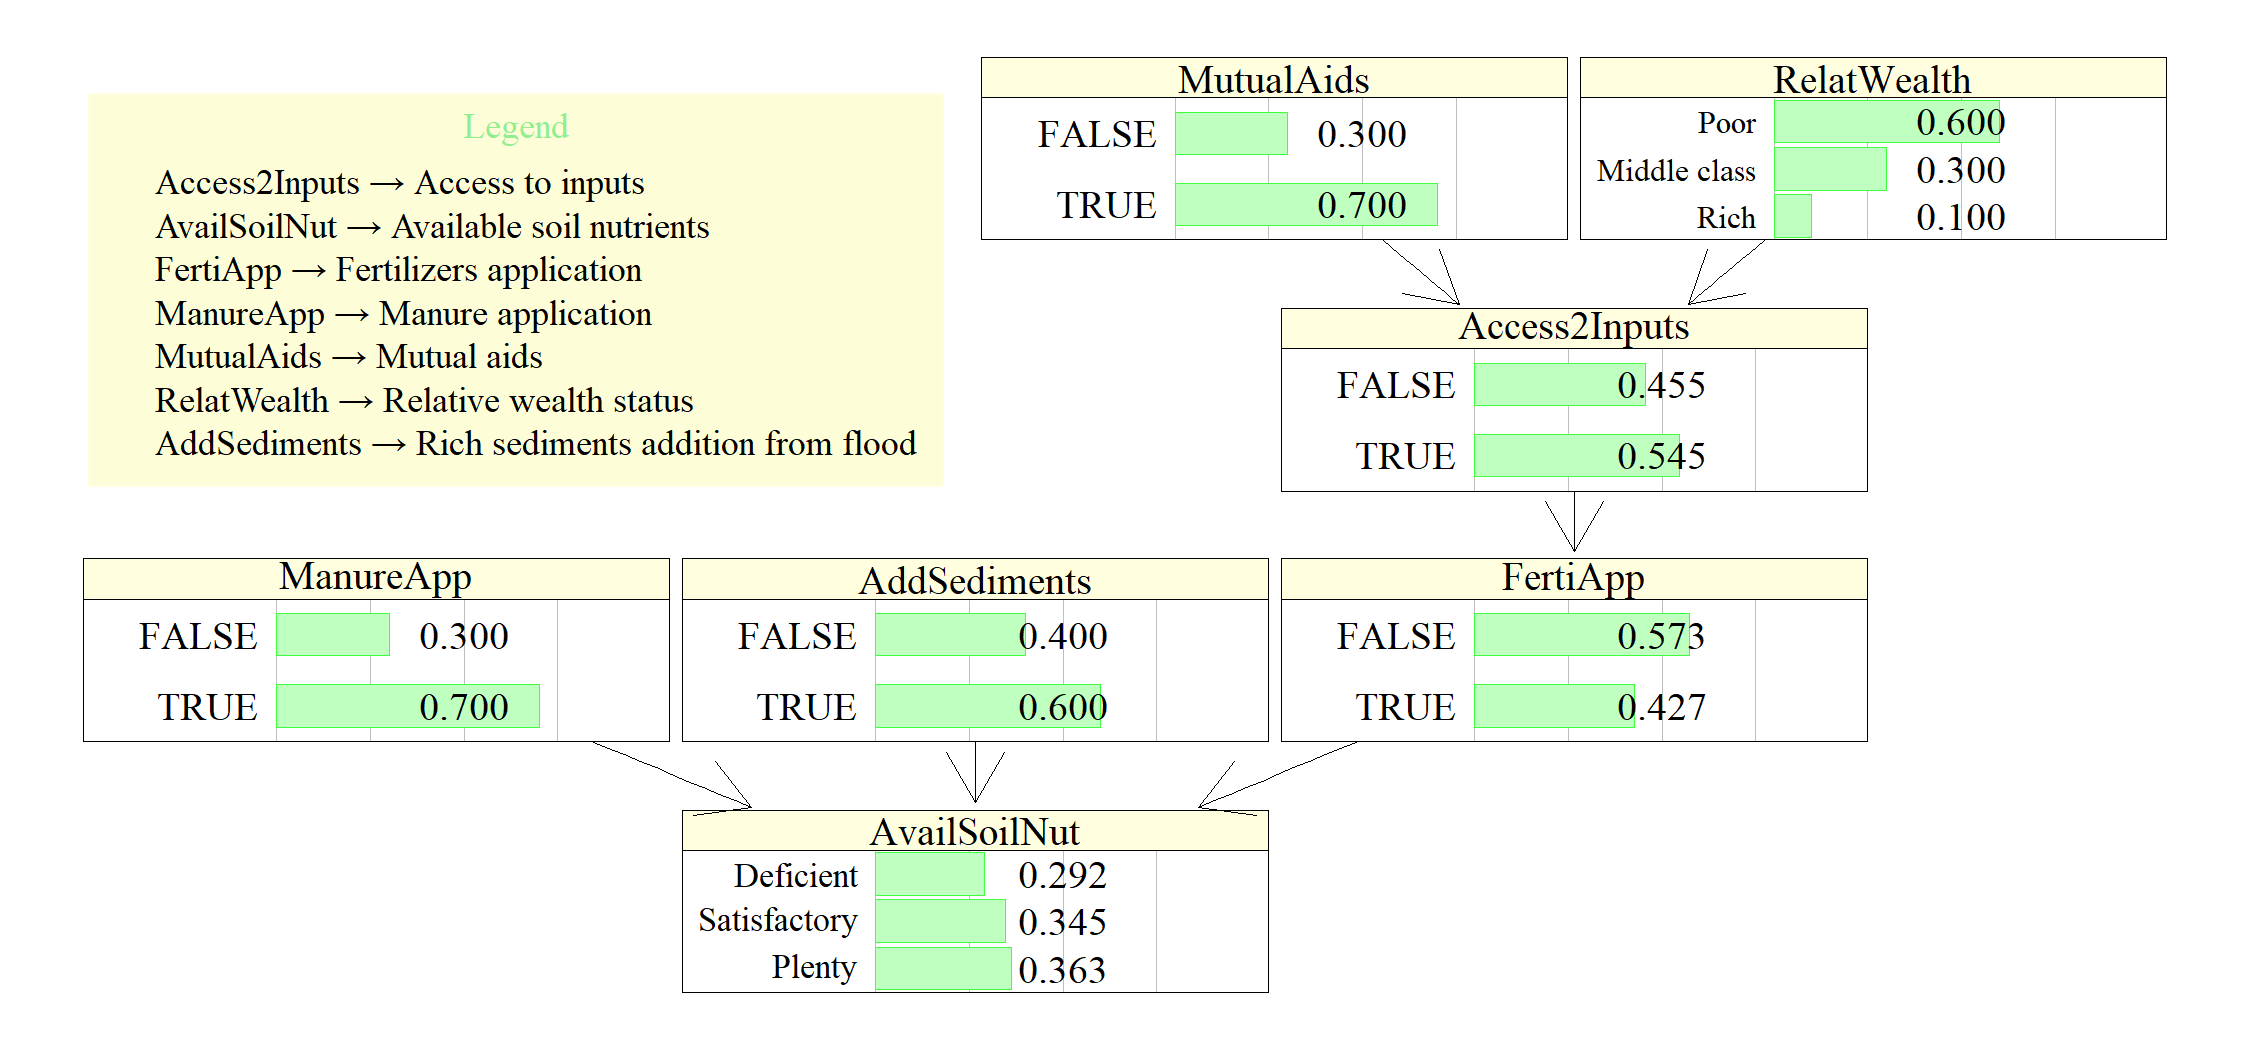
\includegraphics[width=1\linewidth,]{figures/Modelling_FBFS_Available_soil_Nutrients_BNs_plot} 

}

\caption{BNs describing important variables as part of a mixed model describing the available nutrients in FBFS in Kisumu (Kenya) and Tigray (Ethiopia).}\label{fig:fig4}
\end{figure}

The factors that of agricultural management efficiency include the available soil nutrients (AvailSoilNut), crops exposure/sensitivity to pest and diseases (PestDiseaseImpact) and the severity of weeds (WeedsImpact). The magnitude and recurrence of damage to crops due to pests \& diseases and yield losses due to weeds can be related to the skills of the farmers (FarmerSkills) in crop protection, the farmers' ability to acquire chemicals, and other aspects such as the available labour force, which may influence the effectiveness of crop protection.

\begin{figure}[!htbp]

{\centering 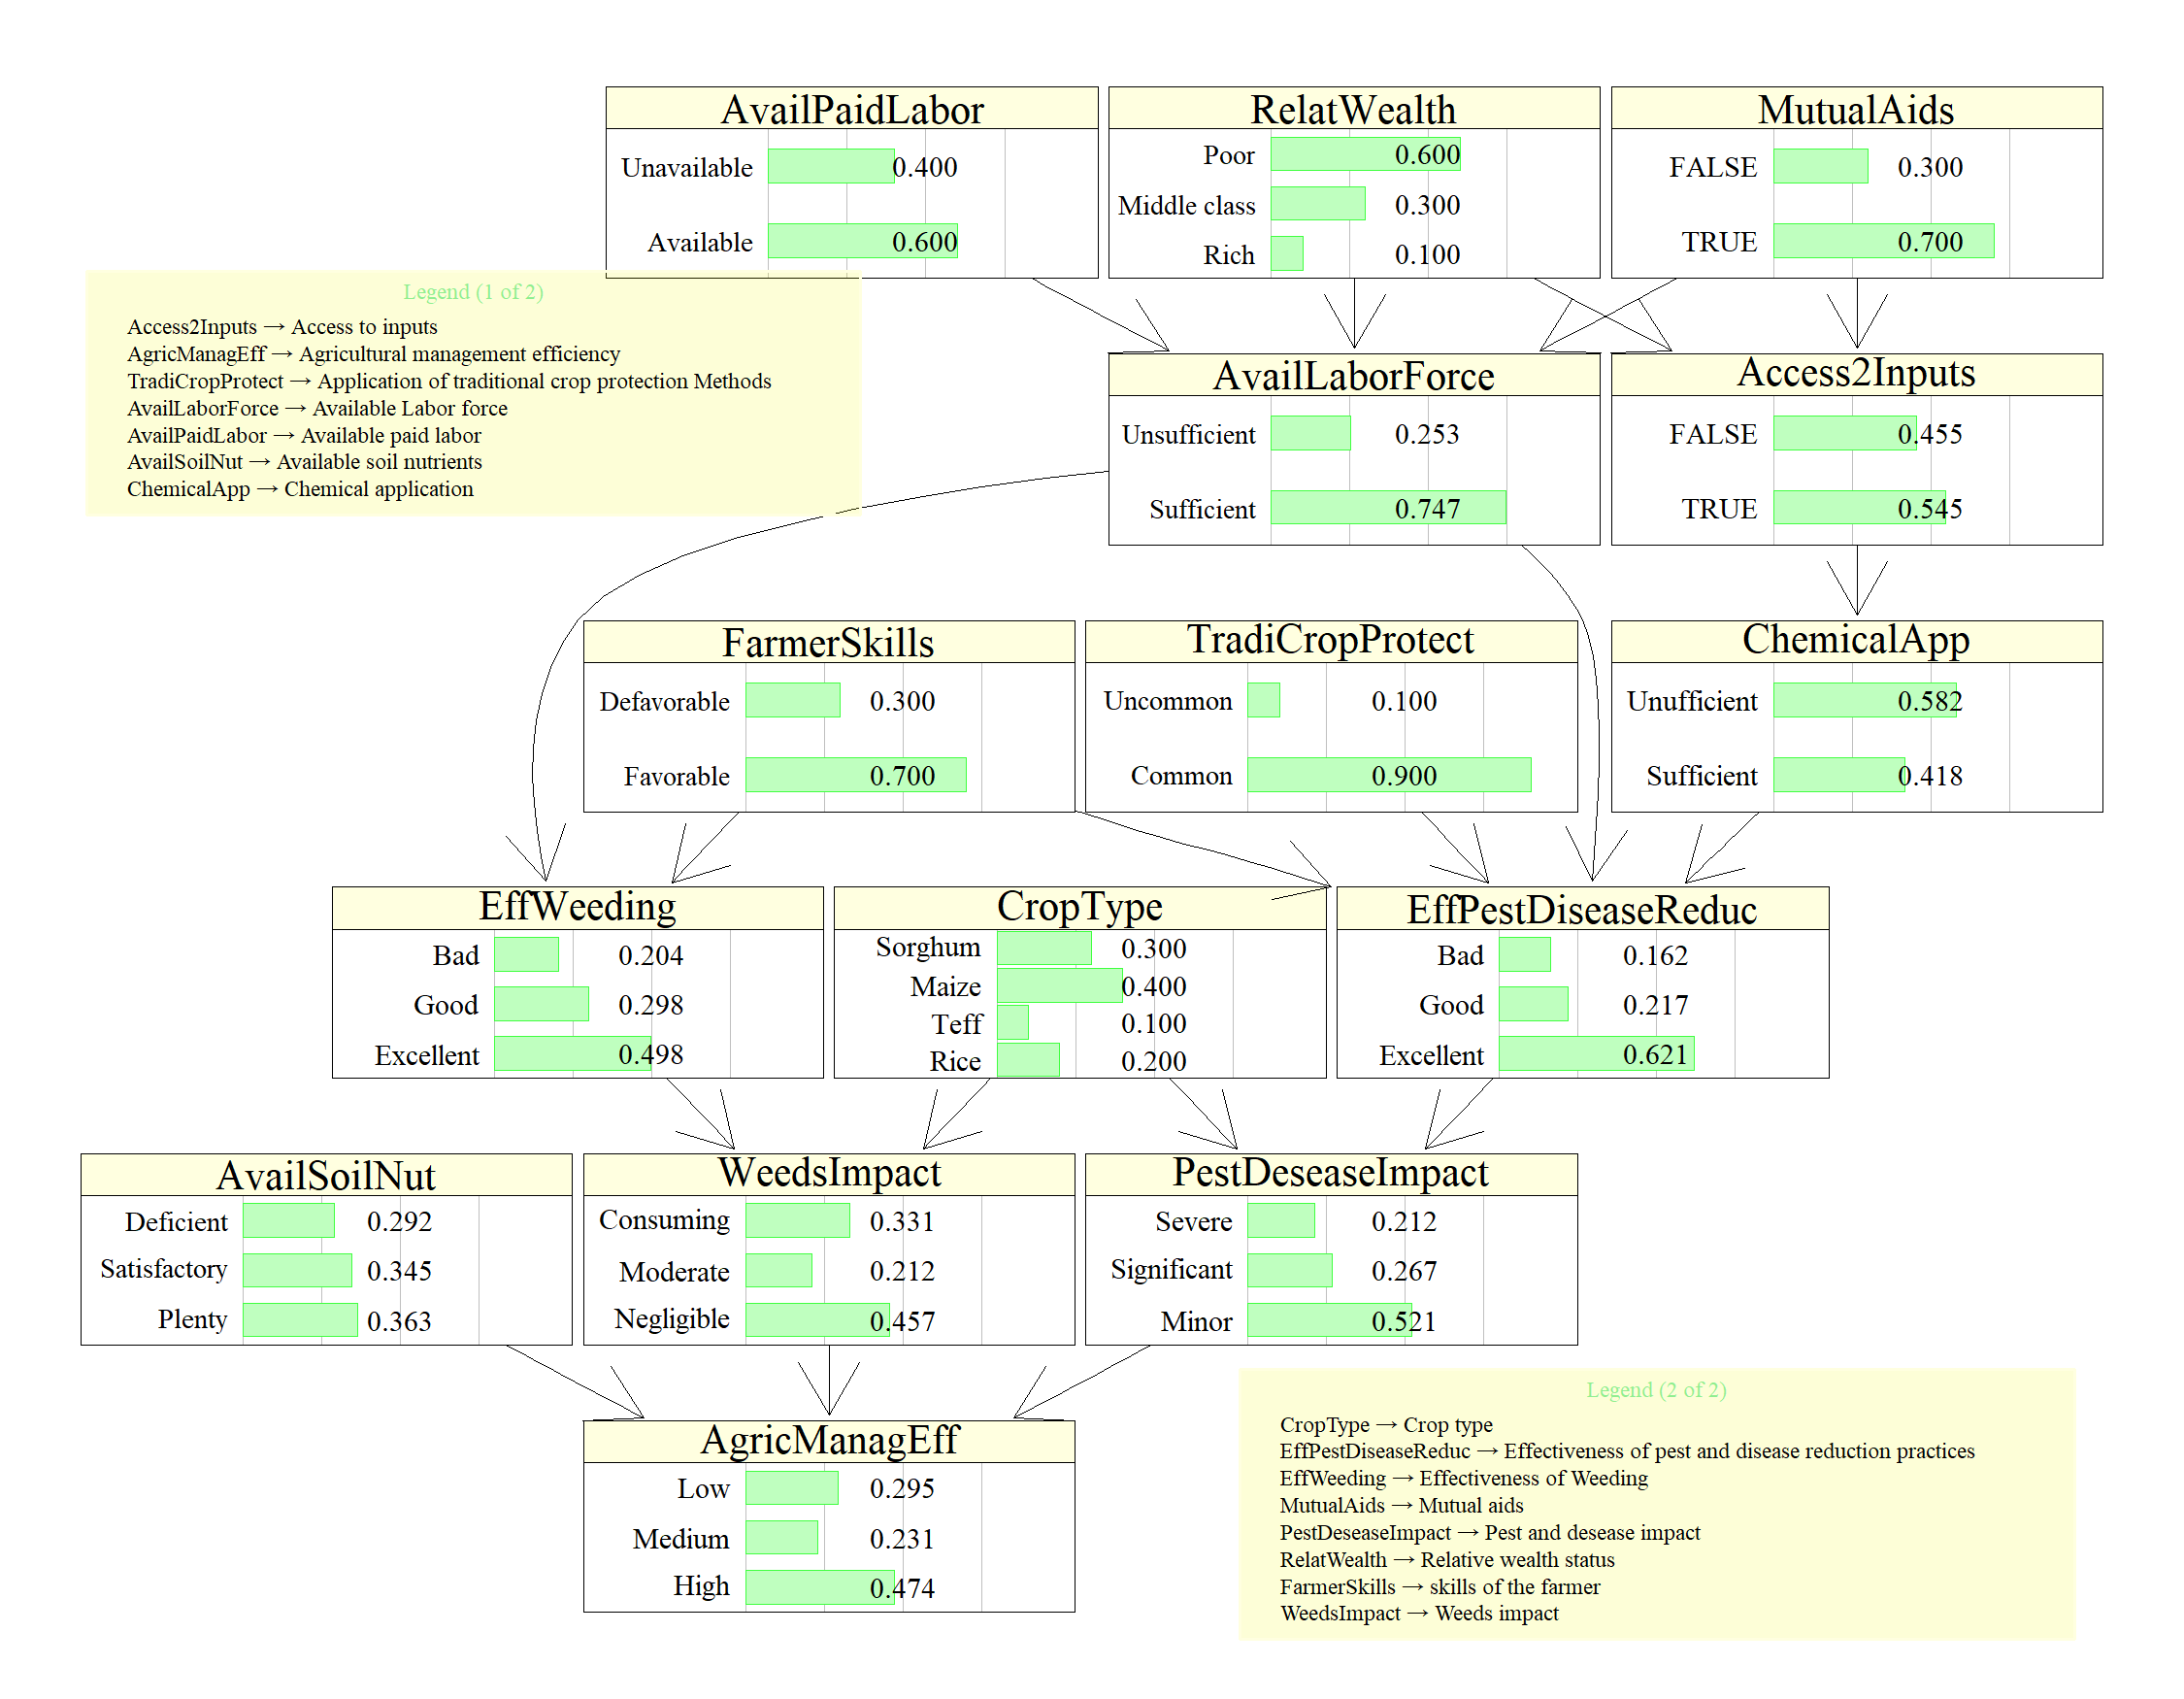
\includegraphics[width=1\linewidth,]{figures/Modelling_FBFS_Agricultural_management_efficiency_BNs_plot} 

}

\caption{BNs describing important variables as part of a mixed model describing the effectiveness of agricultural management in FBFS in Kisumu (Kenya) and Tigray (Ethiopia).}\label{fig:fig5}
\end{figure}

\hypertarget{effectiveness-of-cropping-options-i14}{%
\subsubsection{Effectiveness of cropping options \{\# I14\}}\label{effectiveness-of-cropping-options-i14}}

The effectiveness of cropping options (EffCropsOptions) BN describes the various factors shaping the cropping system at the very early stages of crops growth. Crops are defined by their type (CropType {[}rice, maize, sorghum, teff{]}), their variety (CropVariety) and the farmers' decision regarding which crops to grow and how to grow them (Intercropping). The decision of the farmer to grow a given type of crop and variety have strong implication on yield.

\begin{figure}[!htbp]

{\centering 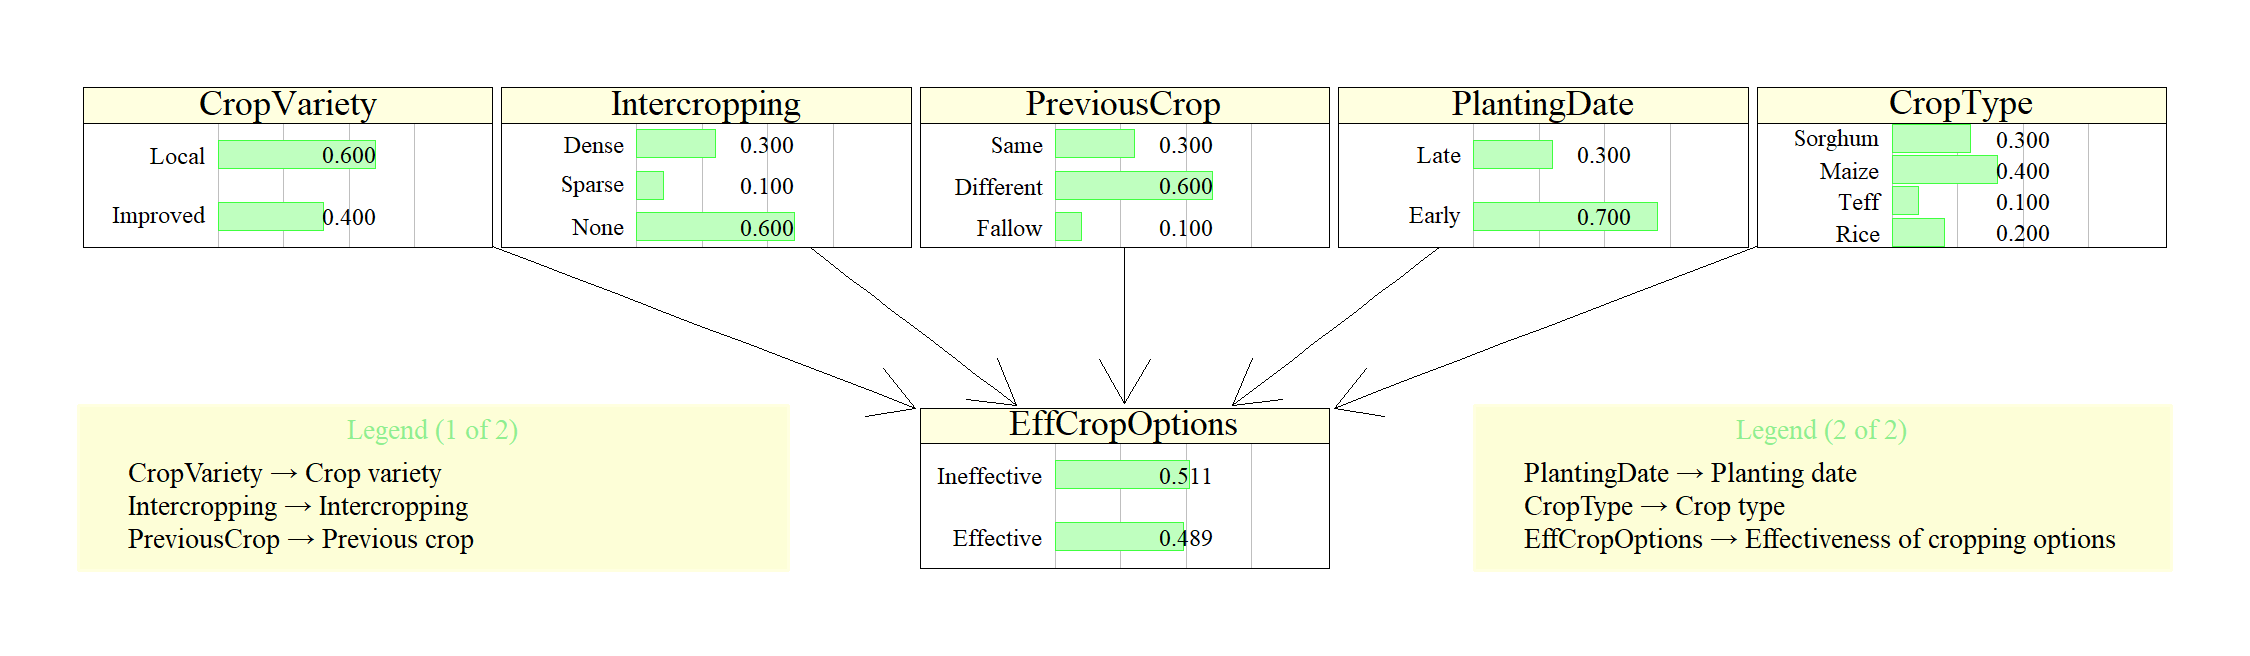
\includegraphics[width=1\linewidth,]{figures/Modelling_FBFS_Suppl_Effectiveness_of_cropping_options_BNs_plot} 

}

\caption{BNs describing important variables as part of a mixed model describing the effectiveness of cropping options in FBFS in Kisumu (Kenya) and Tigray (Ethiopia).}\label{fig:fig6}
\end{figure}

\hypertarget{I15}{%
\subsubsection{BNs structures and nodes sensitivity in relation to crop development}\label{I15}}

In the MC, the whole BNs were replicated with some changes in the CPTs and the causal relations when necessary. for example, the impact of weeds may be different depending on the crop development stages. Our model assumes that crop sensitivity to biotic and abiotic factors depends on the period when these factors are considered. Therefore, these stage-specific BNs or rather the concepts embedded in their nodes, their causal relationships, and their CPTs were made accordingly based on the available source of information. BNs were developed to estimate the farming constraint at plot level and at each phenological stage of crop development. The BN nodes (shown in Figures 5 to 9 are internally represented in four different crop development stages of the model (e.g.~amount of shared flood at initial stage, amount of shared flood at development stage, amount of shared flood at mid stage amount of shared flood at late stage). Few of them that are expected to remain constant over a relatively short period of time (e.g.~the type of water diversion (DiversionType), the slope etc.), however, were represented only once in the model and transported through the various crop development stages. For example, BN nodes soil type and location of the farming plot are considered as static variables as they are unlikely to change, at least not within few years, contrary to other nodes such as the impact of weeds and diseases which differ between consecutive phenological stages. We focus on processes at the initial stage in the description, but the target is assessed quantitively at each of the four stages to feed the MC model.

\hypertarget{I16}{%
\subsubsection{Quantitative assessment of Farming Constraints}\label{I16}}

The best fit for candidate distributions of the target node (farming constraints) derived from the sampling of the posterior probabilities of the BNs are shown in Figure 7. These were fitted to a beta distribution seems owing to the nature of the data (ratio), and the values of the bootstrapped samples lying within reasonable bounds for skewness and kurtosis characterising a reasonable beta function for all the three farming constraints states (low, medium, high). A graphical assessment of the fit including the quantile and probability plots along with the theoretical and empirical density and cumulative distribution functions are presented in Figure 8.

\begin{figure}[!htbp]

{\centering 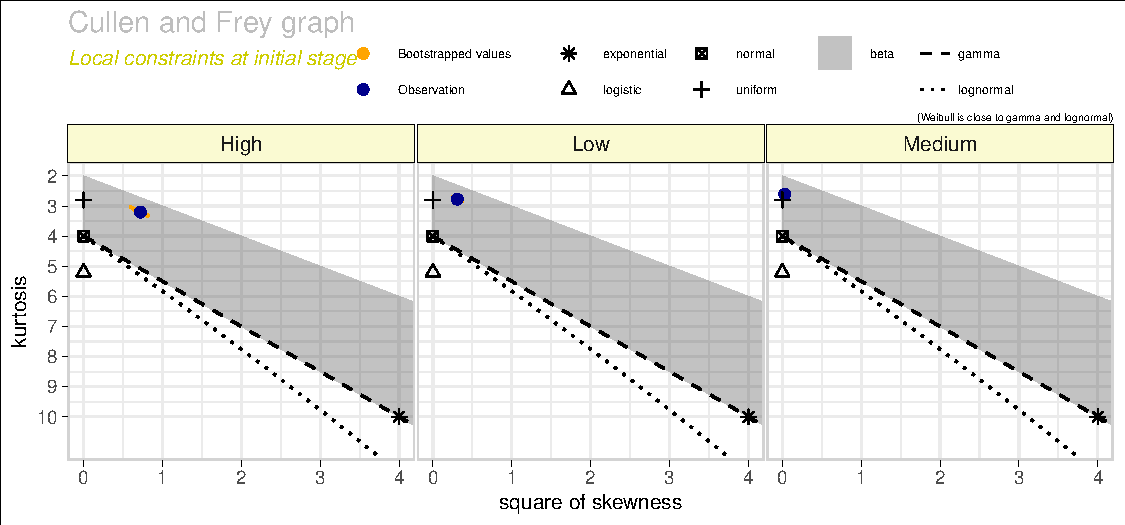
\includegraphics{Modelling_FBFS_Supplement_files/figure-latex/fig7-1} 

}

\caption{Cullen and Frey graph showing the fit of candidate distributions for the joint distribution of the BNs to be used in MC simulation as part of a mixed model describing farming constraints in FBFS in Kisumu (Kenya) and Tigray (Ethiopia) (example for initial stage of crop development).}\label{fig:fig7}
\end{figure}

\begin{figure}[!htbp]

{\centering 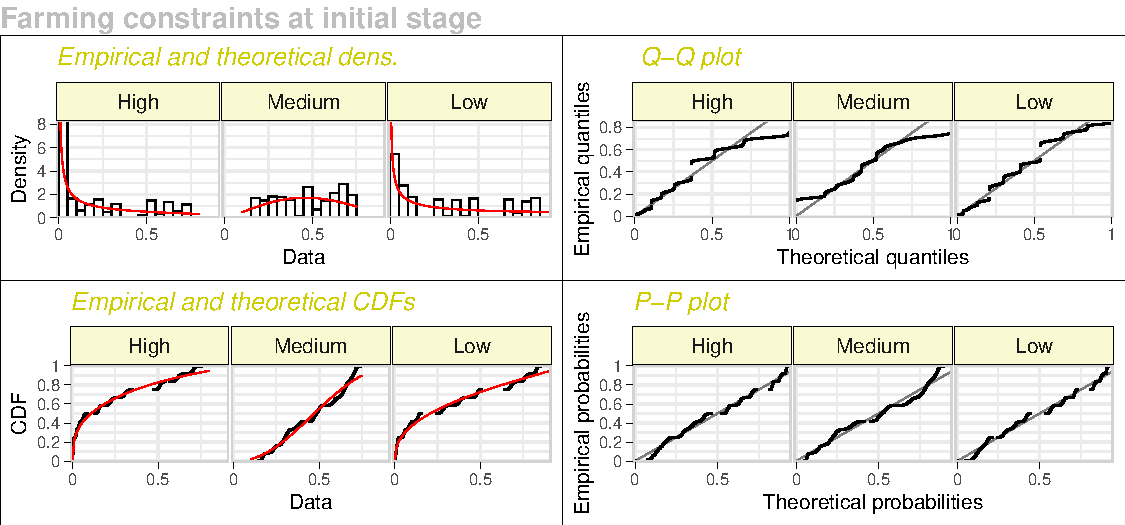
\includegraphics{Modelling_FBFS_Supplement_files/figure-latex/fig8-1} 

}

\caption{Graphical assessment of the fit including the quantile and probability plots along with the theoretical and empirical density and cumulative distribution functions for beta distribution fit assessment as part of a mixed model describing the farming constraints in FBFS in Kisumu (Kenya) and Tigray (Ethiopia) (example for initial stage of crop development).}\label{fig:fig8}
\end{figure}

\hypertarget{I2}{%
\subsection{Model Carlo model}\label{I2}}

As stated earlier, several MC nodes were considered to quantitatively describe crop yield following the 4 development stages considered. Figure 9 presents the graphical model including the initial and development stages. Note that the mid and the late stages were described using the same concept as in the development stage. where a biomass expansion factor (Biomass expansion factor, instead of Average actual yield at initial stage) measuring crop growth potential at a stage (e.g.~Exploitable yield gap (at mid-stage)) and the exploitable yield gap at previous stage (e.g.~Exploitable yield gap (at development stage)) determines the exploitable yield gap at that stage. Potential yield, average actual yield and biomass expansion factor were modelled using gamma distribution, whereas the exploitable yield potential and the harvest index were modelled using uniform distribution.

Figure 9. MC model describing important variables as part of a mixed model describing the expected crop yield at different stages of crop development in FBFS in Kenya and Ethiopia.
We modelled biomass accumulation following the crop development which was ultimately converted into grain yield using a realistic range of harvest index. The maximum attainable biomass yield (Attainable yield potential) depends on the crop potential yield (Yield potential) and its achievable limit (Exploitable yield potential) because it is impossible for farmers to eliminate the farming constraints required for yield potential. The exploitable yield gap (Exploitable yield gap), then, should be estimated by subtracting the long-term average yield (Average actual yield) from the attainable one. Yield opportunity losses (Exploitable yield gap), therefore, is proportional to the difference in inputs allocation among farmers (Farming constraints) relative to the exploitable yield gap. Therefore, additional yield opportunity for a given farmer (Actual exploited yield gap) can be estimated by subtracting the yield opportunity loss from the exploitable yield gap. Finally, farm yield (Expected actual yield) can be obtained by adding the yield opportunity to the average yield.
I.3. Case studies
I.3.1. Qualitative Soil water Assessment under different Management Decisions at initial stage of crop development in Flood-based livelihood systems.

Figure 10. Layout of a 3 x 3 x 2 Split Split-plot experiment with 3 levels of soil type as main plot, 3 different amounts of diverted flood as subplot, and 2 levels of manure application as sub-subplot for studying the available soil water content at initial stage of crop development in FBFS in Kenya and Ethiopia.
Table 1. ANOVA of a Split Split-plot experiment with 3 levels of soil type as main plot, 3 different amounts of diverted flood as subplot, and 2 levels of manure application as sub-subplot for studying the available soil water content at initial stage.
Drought risk

\begin{verbatim}
    Df  Sum Sq  Mean Sq F value Pr(> F)
\end{verbatim}

1 Block 9.00 0.01 0.00 1.04 0.45
2 Soil type 2.00 1.29 0.64 873.66 0.00
3 Manure application 1.00 0.13 0.13 205.41 0.00
4 Soil type:Manure application 2.00 0.04 0.02 27.72 0.00
5 Amount of flood reaching the plot 2.00 1.53 0.77 1972.98 0.00
6 Amount of flood reaching the plot:Soil type 4.00 0.77 0.19 496.27 0.00
7 Amount of flood reaching the plot:Manure application 2.00 0.09 0.05 121.63 0.00
8 Amount of flood reaching the plot:Soil type:Manure application 4.00 0.02 0.01 15.54 0.00

\begin{verbatim}
Normal

    Df  Sum Sq  Mean Sq F value Pr(> F)
\end{verbatim}

9 Block 9.00 0.01 0.00 0.91 0.54
10 Soil type 2.00 1.39 0.69 641.72 0.00
11 Manure application 1.00 0.20 0.20 161.05 0.00
12 Soil type:Manure application 2.00 0.01 0.01 4.14 0.03
13 Amount of flood reaching the plot 2.00 1.48 0.74 899.38 0.00
14 Amount of flood reaching the plot:Soil type 4.00 1.04 0.26 316.91 0.00
15 Amount of flood reaching the plot:Manure application 2.00 0.09 0.05 56.92 0.00
16 Amount of flood reaching the plot:Soil type:Manure application 4.00 0.08 0.02 24.14 0.00

\begin{verbatim}
Waterlogging risk

    Df  Sum Sq  Mean Sq F value Pr(> F)
\end{verbatim}

17 Block 9.00 0.01 0.00 0.76 0.65
18 Soil type 2.00 5.35 2.67 3657.86 0.00
19 Manure application 1.00 0.67 0.67 1365.83 0.00
20 Soil type:Manure application 2.00 0.08 0.04 83.66 0.00
21 Amount of flood reaching the plot 2.00 6.01 3.01 4211.24 0.00
22 Amount of flood reaching the plot:Soil type 4.00 0.02 0.01 7.60 0.00
23 Amount of flood reaching the plot:Manure application 2.00 0.00 0.00 0.14 0.87
Amount of flood reaching the plot:Soil type:Manure application 4.00 0.02 0.00 5.69 0.00

Figure 11. Tukey's HSD test of a Split Split-plot experiment with 3 levels of soil type as main plot, 3 different amounts of diverted flood as subplot, and 2 levels of manure application as sub-subplot for studying the available soil water content at initial stage.
Note: Treatments with the same letter are not significantly different.
I.3.2. Probabilistic Assessment of Biomass Accumulation in Major Crops grown under FBFS in Kisumu, Kenya and Tigray, Ethiopia.
Figure 12. Expected biomass yield and other important yield-related metrics at initial stage of crop development in FBFS in Kenya and Ethiopia.

Figure 13. Expected biomass yield and other important yield-related metrics at late stage of crop development in FBFS in Kenya and Ethiopia.
I.3.3. Case Studies 3: Quantitative grain yield variability and relative performance of Rice and Sorghum under different scenario for water and crop enemies at mid-stage of crop development in flood-based Agriculture.

Figure 14. Layout of a 2 x 2 x 2 x 2 factorial experiment for studying the effects of different level of weeds, pest and diseases and available soil water at mid stage of crop development on grain yield of Sorghum and Rice in FBFS in Kenya and Ethiopia.
Table 2. Effect of different treatments on grain yield of Rice and Sorghum in FBFS in Kenya and Ethiopia.

\begin{verbatim}
term    df  sumsq   meansq  statistic   p.value
\end{verbatim}

1 Pest \& desease 1.00 296634.86 296634.86 41.28 0.00
2 Weeds 1.00 87160.67 87160.67 12.13 0.00
3 Crop type 1.00 93671.65 93671.65 13.04 0.00
4 Available soil water 1.00 1952.71 1952.71 0.27 0.60
5 Pest \& desease:Weeds 1.00 805674.19 805674.19 112.13 0.00
6 Pest \& desease:Crop type 1.00 701930.06 701930.06 97.69 0.00
7 Weeds:Crop type 1.00 99283.33 99283.33 13.82 0.00
8 Pest \& desease:Available soil water 1.00 419006.23 419006.23 58.31 0.00
9 Weeds:Available soil water 1.00 113946.99 113946.99 15.86 0.00
10 Crop type:Available soil water 1.00 612311.35 612311.35 85.22 0.00
11 Pest \& desease:Weeds:Crop type 1.00 863545.62 863545.62 120.18 0.00
12 Pest \& desease:Weeds:Available soil water 1.00 557823.83 557823.83 77.63 0.00
13 Pest \& desease:Crop type:Available soil water 1.00 28012.42 28012.42 3.90 0.05
14 Weeds:Crop type:Available soil water 1.00 34563.49 34563.49 4.81 0.03
15 Pest \& desease:Weeds:Crop type:Available soil water 1.00 516561.41 516561.41 71.89 0.00
16 Residuals 8176.00 58748194.45 7185.44 - -

Note: Available soil water is abbreviated to Soil water. Pest \& disease impact is abbreviated to Pest \& disease.
Table 3. Effect of different treatments levels on grain yield of Rice and Sorghum in FBFS in Kenya and Ethiopia.

\begin{verbatim}
Treatments  diff    lwr upr p.adj
\end{verbatim}

1 Minor:Negligible:Sorghum:Waterlogging-Minor:Negligible:Rice:Drought -92.02 -110.17 -73.86 0.00
2 Severe:Consuming:Sorghum:Waterlogging-Minor:Negligible:Rice:Drought -55.53 -73.69 -37.37 0.00
3 Minor:Consuming:Sorghum:Waterlogging-Minor:Negligible:Rice:Drought -46.92 -65.08 -28.77 0.00
4 Severe:Negligible:Rice:Waterlogging-Minor:Negligible:Sorghum:Drought -46.16 -64.32 -28.00 0.00
5 Minor:Consuming:Rice:Waterlogging-Minor:Negligible:Sorghum:Drought -36.35 -54.51 -18.19 0.00
6 Severe:Negligible:Sorghum:Waterlogging-Minor:Negligible:Rice:Drought -34.45 -52.61 -16.29 0.00
7 Minor:Negligible:Sorghum:Waterlogging-Minor:Consuming:Rice:Drought -34.19 -52.34 -16.03 0.00
8 Minor:Negligible:Sorghum:Waterlogging-Severe:Consuming:Rice:Drought -34.03 -52.18 -15.87 0.00
9 Consuming:Rice:Waterlogging-Negligible:Rice:Drought -31.75 -43.11 -20.40 0.00
10 Severe:Negligible:Rice-Severe:Consuming:Rice -26.88 -38.24 -15.52 0.00
11 Severe:Negligible:Rice-Severe:Negligible:Sorghum -25.32 -36.68 -13.96 0.00
12 Severe:Negligible:Rice-Severe:Consuming:Sorghum -25.06 -36.42 -13.70 0.00
13 Minor:Consuming:Rice:Waterlogging-Minor:Consuming:Rice:Drought -24.9 -43.06 -6.74 0.00
14 Severe:Negligible:Rice:Drought-Minor:Consuming:Rice:Drought -24.32 -42.47 -6.16 0.00
15 Severe:Negligible:Rice:Drought-Severe:Consuming:Rice:Drought -24.15 -42.31 -6.00 0.00
16 Severe:Negligible:Rice:Waterlogging-Severe:Consuming:Sorghum:Drought -23.51 -41.66 -5.35 0.00
17 Negligible:Sorghum:Waterlogging-Negligible:Rice:Drought -22.16 -33.52 -10.80 0.00
18 Negligible:Rice:Waterlogging-Negligible:Rice:Drought -21.62 -32.98 -10.26 0.00
19 Consuming:Rice:Waterlogging-Consuming:Sorghum:Waterlogging -21.6 -32.96 -10.24 0.00
20 Severe:Negligible:Sorghum:Drought-Severe:Consuming:Sorghum:Drought -20.56 -38.71 -2.40 0.01
21 Minor:Consuming:Sorghum:Drought-Severe:Consuming:Sorghum:Drought -20.16 -38.32 -2.01 0.01
22 Severe:Negligible:Rice-Minor:Consuming:Sorghum -19.28 -30.64 -7.93 0.00
23 Severe:Negligible:Rice-Minor:Negligible:Sorghum -18.14 -29.50 -6.79 0.00
24 Severe:Negligible:Rice-Minor:Consuming:Rice -17.06 -28.42 -5.70 0.00
25 Minor:Waterlogging-Minor:Drought -15.28 -22.09 -8.47 0.00
26 Consuming:Rice:Waterlogging-Consuming:Rice:Drought -14.92 -26.27 -3.56 0.00
27 Severe:Waterlogging-Minor:Drought -13.01 -19.82 -6.20 0.00
28 Negligible:Sorghum:Waterlogging-Consuming:Sorghum:Waterlogging -12.01 -23.36 -0.65 0.03
29 Negligible:Rice:Waterlogging-Consuming:Sorghum:Waterlogging -11.46 -22.82 -0.11 0.05
30 Negligible:Waterlogging-Negligible:Drought -8.44 -15.24 -1.63 0.01
31 Consuming:Waterlogging-Negligible:Drought -7.5 -14.31 -0.69 0.02
32 Negligible-Consuming 6.52 2.85 10.20 0.00
33 Rice-Sorghum 6.76 3.09 10.43 0.00
34 Minor:Waterlogging-Severe:Drought 11.06 4.25 17.87 0.00
35 Negligible:Rice-Consuming:Sorghum 13.29 6.48 20.09 0.00
36 Severe:Waterlogging-Severe:Drought 13.33 6.52 20.13 0.00
37 Negligible:Rice-Consuming:Rice 13.49 6.68 20.29 0.00
38 Negligible:Rice-Negligible:Sorghum 13.73 6.92 20.53 0.00
39 Negligible:Drought-Consuming:Drought 13.98 7.18 20.79 0.00
40 Negligible:Sorghum:Waterlogging-Consuming:Sorghum:Drought 15.88 4.52 27.23 0.00
41 Negligible:Rice:Waterlogging-Consuming:Sorghum:Drought 16.42 5.06 27.78 0.00
42 Consuming:Sorghum:Waterlogging-Negligible:Sorghum:Drought 16.75 5.40 28.11 0.00
43 Negligible:Rice:Drought-Consuming:Rice:Drought 16.84 5.48 28.19 0.00
44 Consuming:Rice:Drought-Consuming:Sorghum:Drought 21.2 9.84 32.56 0.00
45 Minor:Negligible:Sorghum:Drought-Severe:Consuming:Sorghum:Drought 22.65 4.50 40.81 0.00
46 Severe:Negligible:Sorghum:Waterlogging-Minor:Consuming:Rice:Drought 23.38 5.22 41.53 0.00
47 Severe:Negligible:Sorghum:Waterlogging-Severe:Consuming:Rice:Drought 23.54 5.38 41.70 0.00
48 Severe:Consuming:Rice:Waterlogging-Minor:Consuming:Sorghum:Drought 26.27 8.11 44.42 0.00
49 Minor:Drought-Severe:Drought 26.34 19.53 33.15 0.00
50 Severe:Consuming:Sorghum:Waterlogging-Severe:Negligible:Rice:Drought 26.61 8.46 44.77 0.00
51 Severe:Consuming:Rice:Waterlogging-Severe:Negligible:Sorghum:Drought 26.66 8.50 44.82 0.00
52 Negligible:Rice:Drought-Negligible:Sorghum:Drought 26.91 15.55 38.27 0.00
53 Consuming:Sorghum:Waterlogging-Consuming:Sorghum:Drought 27.88 16.52 39.24 0.00
54 Minor:Consuming:Sorghum:Waterlogging-Severe:Negligible:Rice:Drought 35.22 17.06 53.38 0.00
55 Minor:Negligible:Rice:Waterlogging-Severe:Consuming:Sorghum:Drought 36.18 18.03 54.34 0.00
56 Negligible:Rice:Drought-Consuming:Sorghum:Drought 38.04 26.68 49.39 0.00
57 Minor:Negligible:Sorghum:Drought-Minor:Consuming:Sorghum:Drought 42.81 24.66 60.97 0.00
58 Minor:Negligible:Sorghum:Drought-Severe:Negligible:Sorghum:Drought 43.21 25.05 61.37 0.00
59 Minor:Negligible:Rice-Severe:Consuming:Rice 44.03 32.68 55.39 0.00
60 Minor:Negligible:Rice-Severe:Negligible:Sorghum 45.59 34.24 56.95 0.00
61 Minor:Negligible:Rice-Severe:Consuming:Sorghum 45.86 34.50 57.21 0.00
62 Severe:Negligible:Sorghum:Waterlogging-Severe:Negligible:Rice:Drought 47.69 29.54 65.85 0.00
63 Minor:Negligible:Rice-Minor:Consuming:Sorghum 51.63 40.28 62.99 0.00
64 Minor:Negligible:Rice-Minor:Negligible:Sorghum 52.77 41.42 64.13 0.00
65 Minor:Negligible:Rice-Minor:Consuming:Rice 53.85 42.50 65.21 0.00
66 Minor:Negligible:Rice:Waterlogging-Minor:Consuming:Sorghum:Drought 56.34 38.19 74.50 0.00
67 Minor:Negligible:Rice:Waterlogging-Severe:Negligible:Sorghum:Drought 56.74 38.58 74.90 0.00
68 Minor:Negligible:Rice:Drought-Minor:Consuming:Rice:Drought 57.83 39.67 75.98 0.00
69 Minor:Negligible:Rice:Drought-Severe:Consuming:Rice:Drought 57.99 39.83 76.15 0.00
70 Minor:Negligible:Rice-Severe:Negligible:Rice 70.92 59.56 82.27 0.00
71 Minor:Negligible:Rice:Drought-Severe:Negligible:Rice:Drought 82.14 63.99 100.30 0.00

Table 4. Comparative analysis of joint effects of different treatments levels on grain yield of Rice and Sorghum in FBFS in Kenya and Ethiopia.

\begin{verbatim}
    Grain yield groups
\end{verbatim}

1 Minor:Negligible:Rice:Drought risk 166.0966 a
2 Minor:Negligible:Rice:Waterlogging risk 133.2508 b
3 Severe:Negligible:Sorghum:Waterlogging risk 131.6462 b
4 Minor:Negligible:Sorghum:Drought risk 119.7207 bc
5 Minor:Consuming:Sorghum:Waterlogging risk 119.1722 bc
6 Severe:Consuming:Sorghum:Waterlogging risk 110.5669 cd
7 Minor:Consuming:Rice:Drought risk 108.2687 cd
8 Severe:Consuming:Rice:Drought risk 108.1058 cd
9 Severe:Consuming:Rice:Waterlogging risk 103.1724 cd
10 Severe:Consuming:Sorghum:Drought risk 97.06859 de
11 Severe:Negligible:Rice:Drought risk 83.95261 ef
12 Minor:Consuming:Rice:Waterlogging risk 83.3691 ef
13 Minor:Consuming:Sorghum:Drought risk 76.90688 f
14 Severe:Negligible:Sorghum:Drought risk 76.51145 f
15 Minor:Negligible:Sorghum:Waterlogging risk 74.0806 f
16 Severe:Negligible:Rice:Waterlogging risk 73.56149 f

Note: treatments with the same letters are not statistically significantly different. Colon (:) between levels of the different treatments denote interactions. Minus (-) between interacting levels of different traitment denonte

\hypertarget{VI}{%
\section{reference}\label{VI}}


\end{document}
